\documentclass[conference]{IEEEtran}

% *** GRAPHICS RELATED PACKAGES ***
%
\usepackage[pdftex]{graphicx}


% *** MATH PACKAGES ***
%
\usepackage{amsmath}
\usepackage{mathtools}
\DeclarePairedDelimiter\floor{\lfloor}{\rfloor}

% *** SUBFIGURE PACKAGES ***
\ifCLASSOPTIONcompsoc
 \usepackage[caption=false,font=normalsize,labelfont=sf,textfont=sf]{subfig}
\else
 \usepackage[caption=false,font=footnotesize]{subfig}
\fi


% *** PDF, URL AND HYPERLINK PACKAGES ***
%
\usepackage{url}


\usepackage[brazilian]{babel}
\usepackage[utf8]{inputenc}
%\usepackage[T1]{fontenc}
\usepackage{fancyhdr}


% correct bad hyphenation here
%\hyphenation{op-tical net-works semi-conduc-tor}


\pagestyle{fancy}
%\fancyhf{}
\chead{VII Workshop de P\'{o}s-Gradua\c{c}\~{a}o - Engenharia de Computa\c{c}\~{a}o - WPGEC 2018}
\renewcommand{\headrulewidth}{2pt}

\pagenumbering{gobble}

\begin{document}


\title{Glaucoma diagnostic using nerve fiber layer thickness images \\ Diagnóstico do glaucoma a partir de imagens de espessuras da camada de fibras nervosas}


\author{\IEEEauthorblockN{BRAGA, Samira J.\IEEEauthorrefmark{1};
GOMI, Edson S.\IEEEauthorrefmark{1}}
\IEEEauthorblockA{\IEEEauthorrefmark{1}Escola Politécnica da Universidade de São Paulo}}


% make the title area
\maketitle

\thispagestyle{fancy}

\renewcommand{\abstractname}{Abstract}
\begin{abstract}
Abstract here.
\end{abstract}

\renewcommand\IEEEkeywordsname{Keywords}
\begin{IEEEkeywords}
\label{Keywords}
word 1; word 2.
\end{IEEEkeywords}

\renewcommand{\abstractname}{Resumo}
\begin{abstract}
\label{Resumo}
\'E necess\'aria a inser\c{c}\~{a}o do resumo para artigo escrito em Portugu\^{e}s.
\end{abstract}

\renewcommand\IEEEkeywordsname{Palavras-chave}
\begin{IEEEkeywords}
\label{Palavras-chave}
palavra 1; palavra 2.
\end{IEEEkeywords}

\renewcommand\IEEEkeywordsname{Classifica\c{c}\~{a}o}
\begin{IEEEkeywords}
	\label{classificacao}
	Mestrado
\end{IEEEkeywords}

\renewcommand\IEEEkeywordsname{Categoria}
\begin{IEEEkeywords}
	\label{Categoria}
	Iniciante 
\end{IEEEkeywords}

\IEEEpeerreviewmaketitle


\section{Introdução}

%avaliação da espessura numa area mais extensa (nao só no circulo) melhora a capacidade de diagnostico?

Glaucoma é uma neuropatia óptica crônica multifatorial e de lenta progressão que causa perda de campo visual. Pesquisa realizada por Quigley e Broman mostrou que glaucoma é a segunda maior causa de cegueira no mundo e estimaram que atingirá 79,6 milhões de pessoas até 2020 \cite{Quigley2006}. O glaucoma caracteriza-se pela perda da camada de fibras nervosas no olho, o que pode causar cegueira se não for tratada corretamente \cite{Quigley2011}. O dano na camada de fibras nervosas acontece antes de alteração no campo visual do paciente e, por isso, o diagnóstico precoce é um fator importante para evitar a perda da visão \cite{Malik2012}.

O objetivo deste trabalho é investigar se é possível fazer o diagnóstico do glaucoma a partir das imagens da espessura da camada de fibras nervosas por meio de uma rede convolucional.

\section{Diagnóstico de glaucoma}

%o que e glaucoma (tese marcelo)
%como e feito o diagnostico
%oct no diagnostico

\begin{figure}[!tp]
  \centering
  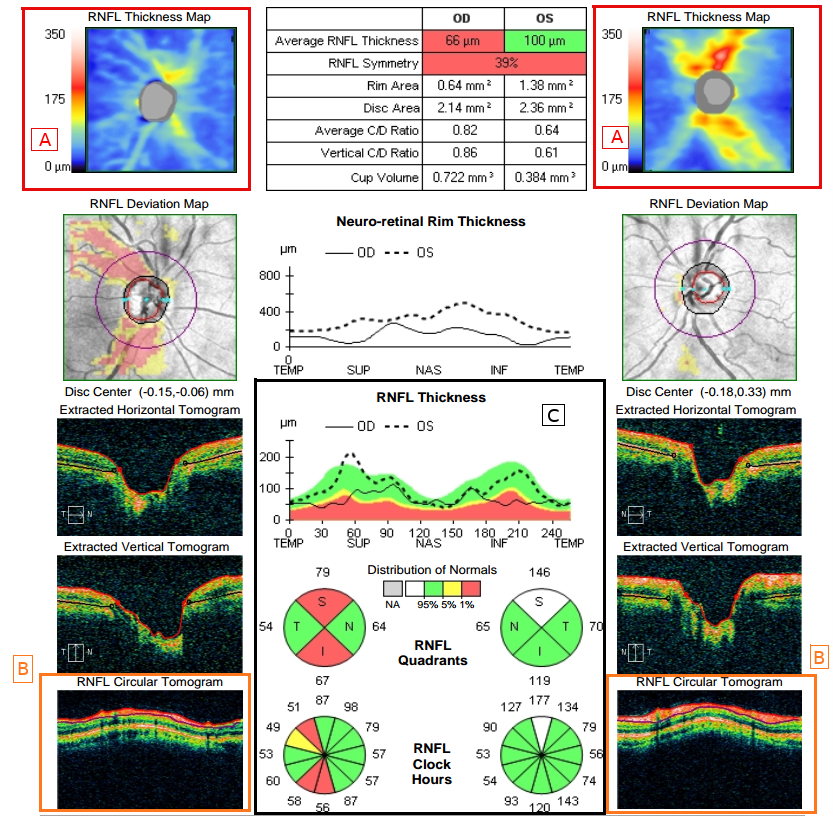
\includegraphics[width=2.5in]{img/oct_regiao.png}
  \caption{Saída de um exame de OCT.}
  \label{fig:oct}
\end{figure}

\begin{figure*}[!t]
  \centering
  \subfloat[Imagem de entrada da rede]{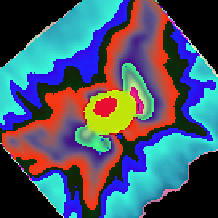
\includegraphics[width=1in]{img/conv/data}%
  \label{fig:data}}
  \hfil
  \subfloat[Imagem de saída da primeira camada convolucional]{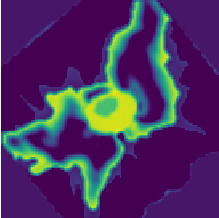
\includegraphics[width=1in]{img/conv/conv1_1}%
  \label{fig:conv1}}
  \hfil
  \subfloat[Imagem de saída da segunda camada convolucional]{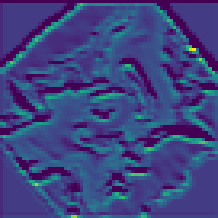
\includegraphics[width=1in]{img/conv/conv2_1}%
  \label{fig:conv2}}
  \hfil
  \subfloat[Imagem de saída da terceira camada convolucional]{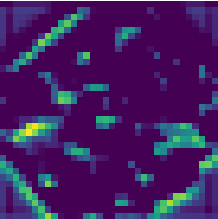
\includegraphics[width=1in]{img/conv/conv3_1}%
  \label{fig:conv3}}
  \hfil
  \subfloat[Imagem de saída da quarta camada convolucional]{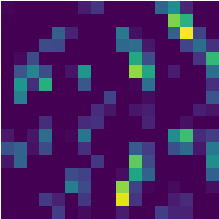
\includegraphics[width=1in]{img/conv/conv4_1}%
  \label{fig:conv4}}
  \hfil
  \subfloat[Imagem de saída da quinta camada convolucional]{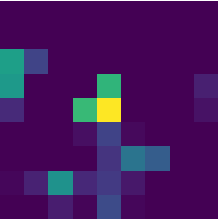
\includegraphics[width=1in]{img/conv/conv5_1}%
  \label{fig:conv5}}
  \caption{Exemplos de saídas de cada camada convolucional ao longo da rede.}
  \label{fig:imagens_rede}
\end{figure*}

%referencia para OCT e para SAP ****** OK

Atualmente, o diagnóstico do glaucoma é feito com uma combinação de exame estrutural, por meio de tomografia de coerência óptica OCT (Optical Coherence Tomography) \cite{Wollstein2005}, e exame funcional, por meio da perimetria computadorizada SAP (Standard Automated Perimetry) \cite{chauhan1990}. Os exames estruturais avaliam a camada de fibras nervosas para identificar alterações na sua espessura e os exames funcionais avaliam o campo visual do paciente em busca de áreas de perda da visão. 

%Não é simples identificar a existência do glaucoma antes que haja dano ao campo visual \cite{Populacoes2009}. 
O exame OCT utiliza o princípio da interferometria luminosa para medir as espessuras das estruturas intraoculares. Ao realizar uma varredura, o equipamento emite feixes de laser infravermelho e mede o tempo que a luz leva para ser refletida. Em cada estrutura atravessada, uma parte dessa luz é refletida de volta. O cálculo da espessura é baseado na diferença entre o feixe de luz de referência e a luz refletida \cite{huang1991}. 

% arrumar explicação *************** OK
Na figura \ref{fig:oct} vemos a saída gerada pelo equipamento Cirrus HD-OCT da Carl Zeiss Meditec Inc. Na região A, indicada em vermelho, está as imagens de espessuras da camada de fibras nervosas. Essas espessuras são representadas como em um mapa de calor, onde espessuras próximas à $0$ são apresentadas em azul, do verde até o amarelo e laranja são espessuras até $175$ mícrons e de vermelho até aproximar-se do branco representam espessuras de $175$ à $350$ mícrons. O disco central em cinza é a fóvea, ponto cego do olho de onde sai o nervo óptico. Na região B, em laranja, são exibidas as imagens tomográficas da camada de fibras nervosas em um corte circular em volta da fóvea. A região C, em preto, exibe gráficos de espessura na região circular ao redor da fóvea, também chamada de mapa TSNIT (Temporal, Superior, Nasal, Inferior, Temporal). Além do gráfico, são exibidos também as médias de espessura por quadrantes e horas de relógio. As medidas de espessuras são sempre comparadas com o banco de dados normativo do aparelho para indicar se a medida está dentro de 95\% da população normal (em verde), dentro de apenas 5\% da população (em amarelo), ou em apenas 1\% da população (em vermelho) \cite{aref2010}. 

%medico precisa ter especializacao para avaliar e dar o diagnostico *********** OK
%auxiliar na tomada de decisão **************** OK
O estudo de Gracitelli \textit{et al.} mostra que os parâmetros de média de espessura por quadrantes ou a média global da espessura da camada de fibras nervosas é amplamente utilizado na análise para diagnóstico do glaucoma \cite{Gracitelli2015}. No entanto, nenhum exame fornece resultados definitivos da situação do paciente, necessitando assim da avaliação de um profissional oftalmologista especialista em glaucoma para conclusão do resultado. Esta análise não é padronizada e pode variar de acordo com o julgamento do oftalmologista \cite{kroese2003}. É possível utilizar classificadores de aprendizagem de máquina para auxiliar na tomada de decisão do oftalmologista. Um classificador de rede neural profunda foi utilizado com dados de exame de campo visual para detectar estágios iniciais de glaucoma \cite{Asaoka2016}. Dados de OCT e SAP em conjunto também foram utilizados para treinar diversos tipos de classificadores \cite{Populacoes2009,bowd2008}. Em geral, equipamentos oftalmológicos possuem seus próprios algoritmos para análise e classificação, mas o estudo de Kwokleung Chan \textit{et al.} mostra que algoritmos de classificação são mais eficientes \cite{kwokleung2002}.

% classificadores com parametros de oct (horas de relogio) e sap
%pegar imagem do oct para utilizar toda a area de espessura do nervo para usar no diagnostico

\section{Redes neurais convolucionais}

%o que sao redes convolucionais
%explicar cada tipo de camada
%imagens das saidas em cada convolucional

Redes neurais profundas estão sendo amplamente utilizadas em diversos domínios para classificação e detecção de objetos, principalmente em visão computacional e reconhecimento e processamento de linguagem natural. Essas redes consistem em várias camadas conectadas que aprendem a reconhecer padrões nos dados apresentados, sejam eles imagens ou sons \cite{LeCun2015}. O principal tipo de rede utilizado é a rede neural convolucional CNN (Convolutional Neural Network). As CNNs mostraram ser excelentes ferramentas no processamento de imagens, inclusive na área médica, sendo utilizadas para classificação, detecção de objetos e segmentação. Esse sucesso deve-se principalmente à utilização de grandes quantidades de exemplos de treinamento, que permitem que a rede aprenda a reconhecer características a partir dos dados brutos das imagens \cite{greenspan2016}. %raw data?

As CNNs são compostas de várias camadas conectadas, sendo os principais tipos as convolucionais, pooling e as camadas totalmente conectadas. As camadas convolucionais servem como filtros para identificar as características das imagens, como curvas, bordas e cores. As saídas das camadas convolucionais são mapas de características identificadas na imagem de entrada. A convolução é feita utilizando uma máscara (ou kernel) que desliza por todos os pixels da imagem multiplicando os valores do pixel pelos valores da máscara. Essa multiplicação é feita em toda a imagem com diferentes máscaras, gerando assim as saídas dos diferentes filtros em cada camada de convolução.

Após a identificação dessas características, a camada de pooling agrupa as características e reduz a resolução da imagem. Também utilizando uma máscara, a operação de pooling irá calcular o valor máximo em cada região da imagem, agrupando características similares em um mesmo pixel. Na figura \ref{fig:imagens_rede} é possível acompanhar o agrupamento de características e a redução da resolução da imagem ao longo de 5 camadas convolucionais e pooling.

As camadas totalmente conectadas recebem todas as características identificadas nas imagens e fazem a classificação final. A saída dessa camada será um vetor com o número de classes a serem classificadas, cada classe terá um valor de probabilidade sendo o maior valor a classe identificada para a imagem. O desenho de uma configuração de rede convolucional profunda pode ser visto na figura \ref{fig:convolucao}. Várias camadas de convolução e pooling utilizando ativações por ReLU (Rectified Linear Unit) são seguidas por duas ou mais camadas totalmente conectadas. O aumento da quantidade de camadas mostrou-se eficiente no aumento da acurácia de classificação das redes convolucionais \cite{simonyan2014}.

%referencia imagem ****** OK

\begin{figure}[!tp]
 \centering
 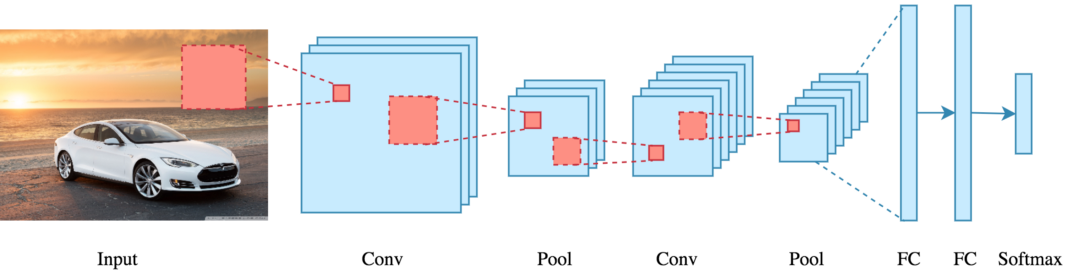
\includegraphics[width=3in]{img/convolucao.png}
 \caption{Esquema de camadas de uma rede neural convolucional \cite{convTDS}.}
 \label{fig:convolucao}
\end{figure}


  \subsection{Transfer Learning}

  %como e feito transfer learning
  %tecnicas: fine tuning, feature extraction
  %utilizacao em saude

  %dar exemplo do treinamento do VGG ****** OK
  Para treinar uma CNN é necessário ter um conjunto muito grande de exemplos para treinamento e teste. As redes VGG, por exemplo, foram treinadas utilizando o dataset ILSVRC-2012 \cite{ILSVRC15} que contém 1000 classes e foi dividido em 3 conjuntos: 1.3 milhões de imagens para treino, 50 mil imagens para validação e 100 mil imagens para teste \cite{simonyan2014}. No entanto, imagens médicas são muito mais difíceis de se obter, principalmente com anotações de classes, devido ao tempo para realizar os estudos e para anotar todos os exemplos \cite{greenspan2016}.
  
  Uma alternativa para a utilização de redes profundas com um dataset menor é a utilização do transfer learning. Essa técnica consiste em usar uma rede treinada com um dataset grande de imagens em um domínio mais amplo e transferir esse conhecimento para um domínio mais específico. Dessa forma, ao invés de utilizar inicialização randômica dos parâmetros da rede, utiliza-se os pesos de uma rede já treinada. A utilização de uma rede pré-treinada reduz o tempo de treinamento e a necessidade de um dataset muito grande para o novo objetivo \cite{tan2018}.

  A aplicação do transfer learning pode ser feita em diversos contextos onde haja dificuldade de obter dados para treinamento. Em um survey, Shao \textit{et al.} \cite{shao2015} relatam diversos usos de transfer learning para treinamento de redes com diferentes domínios alvo. Em oftalmologia, essa técnica mostrou-se eficiente para classificação de retinopatia diabética \cite{li2017} e degeneração macular \cite{lee2017}. Nestes trabalhos foram utilizadas redes pré-treinadas com o dataset ImageNet, o que mostra que é possível utilizar o conhecimento de um domínio de origem mais amplo em uma tarefa específica. 

  \subsection{Redes pré-treinadas}

  %explicar vgg

  Entre as diversas redes convolucionais já treinadas com o ImageNet, foi escolhida a rede VGG16 para utilização neste experimento. Essa rede foi utilizada para classificação de degeneração macular com imagens de OCT no estudo de Lee \textit{et al.} \cite{lee2017}. Os resultados apresentados são promissores, obtendo área sob a curva ROC de $97,46\%$.

  A rede VGG16 foi utilizada no ImageNet Large Scale Visual Recognition Challenge (ILSVRC) em 2014, uma competição de reconhecimento de imagens utilizando redes neurais profundas. A rede é composta ao todo de $21$ camadas com ativações ReLU, sendo $13$ camadas convolucionais, $5$ max pooling e $3$ camadas totalmente conectadas no final, duas com 4096 saídas e a última com 1000 saídas de classificação. Diferente de outras arquiteturas, o VGG16 utiliza kernels menores nas camadas de convolução, o que diminui o número de pesos necessários mas ainda com um poder discriminativo alto. \cite{simonyan2014}.

\section{Experimentos e resultados}

  \subsection{Dataset}

  %aumento do dataset, rotações aleatorias entre 0 e 360
  %divisao treino e validação

  O dataset original foi obtido com o departamento de oftalmologia da Unicamp. O dataset consiste de imagens de OCT com tamanho 136x136 de $56$ olhos com glaucoma e $66$ olhos normais, totalizando $122$ pacientes. As imagens de espessura da camada de fibras nervosas foram obtidas através da extração das imagens do PDF do exame. Foram selecionados para o experimento somente os olhos de pacientes que foram manualmente classificados por especialistas.

  Para a separação do dataset em treino e validação, foram selecionados $20\%$ de olhos normais e $20\%$ de olhos com glaucoma para validação, e o restante para treino, totalizando $98$ imagens de treino e $24$ para validação. As imagens selecionadas para teste não estão presentes no dataset de treino, para que o algoritmo possa classificar imagens independentes.

  Para evitar overfitting, foi empregada uma técnica para aumentar o número de exemplos a partir das imagens no dataset de treino. Cada imagem foi rotacionada $100$ vezes em ângulos aleatórios entre $0$ e $360$ graus, gerando assim um dataset de treino com $9800$ imagens. As imagens de validação não foram rotacionadas.

  \subsection{Pré-processamento}

  % subtração da media
  % areas pretas para zero absoluto

  %formula do calculo do pixel medio
  
  %gerar saida da imagem media, calcular desvio padrao, gerar imagens com media+desvio padrao e media-desvio padrao
  
  Para utilização do transfer learning, foi necessário fazer a subtração do pixel médio. O pixel médio é calculado sobre todas as imagens do dataset de treino utilizando a equação \ref{eq:mean_pixel}, onde $P_c$ é o valor médio por canal, $M$ e $N$ são as dimensões das imagens de entrada (largura e altura, respectivamente), $I$ é a quantidade total de imagens no dataset de treino e $p_{mni}$ é o valor do pixel na posição $\{m,n\}$ na imagem $i$. O valor do pixel médio é calculado em cada canal RGB da imagem, gerando assim um vetor de 3 posições com um valor médio por canal.

  %verificar equacao *********************

  \begin{equation}
    P_c = \frac{1}{M * N * I} \sum p_{mni}
    \label{eq:mean_pixel}
  \end{equation}

%exemplo imagem com falha *************** OK
  % Onde houveram falhas na aquisição da imagem gerando áreas escuras, como no exemplo da figura \ref{fig:exemplo_falha}, pixels com valores RGB próximos ao preto foram substituídos pelo valor de preto absoluto RGB (0, 0, 0) **para que não tenham influência sobre a decisão do classificador**.

  % \begin{figure}[!tp]
  %   \centering
  %   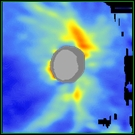
\includegraphics[width=1.2in]{img/falha.png}
  %   \caption{Exemplo de imagem onde houve falha na aquisição, gerando as áreas pretas no lado direito.}
  %   \label{fig:exemplo_falha}
  % \end{figure}

  \subsection{Resultados com transfer learning}

  %estrategia de learning rate
  %iterações e tempo de processamento
  %grafico da acuracia

  \begin{figure}[!tp]
    \centering
    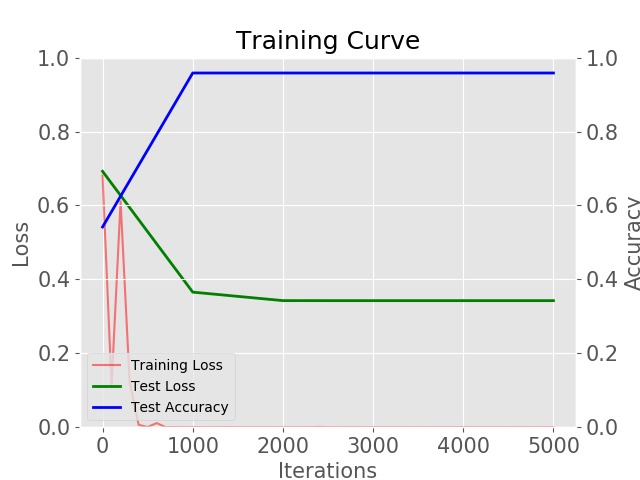
\includegraphics[width=2.5in]{img/curve_vgg16.png}
    \caption{Acurácia e erro de treino e validação da rede VGG16 com transfer learning.}
    \label{fig:acuracia_vgg16_transfer}
  \end{figure}


  Neste experimento, foi utilizada a mesma arquitetura da rede VGG16, alterando a saída da última camada totalmente conectada para duas saídas, correspondente às duas classes a serem classificadas: normal e glaucoma. Os pesos pré-treinados foram carregados para inicialização apenas das camadas convolucionais. As três últimas camadas totalmente conectadas foram inicializadas com valores aleatórios de uma distribuição normal com desvio padrão $0.01$. %As imagens do Imagenet tinham a resolução de 224x224 pixels, enquanto que as imagens de OCT têm resolução de 136x136 pixels, por isso a camada de entrada da rede também foi alterada para a resolução das imagens do dataset utilizado.
  
  O treinamento foi realizado em todas as camadas da rede, utilizando o gradiente descendente estocástico por $5000$ iterações, com mini batches de $15$ imagens. Os parâmetros de momentum e weight decay foram definidos como $0.9$ e $0.0005$, respectivamente. A taxa de aprendizagem inicial foi de $0.001$. A cada $1000$ iterações a taxa de aprendizagem foi diminuída utilizando a equação \ref{eq:learning_rate}. Onde $base\_lr$ é a taxa de aprendizagem inicial, $\gamma$ é um parâmetro definido com o valor $0.1$, $iter$ é o número da iteração atual e $step$ é um parâmetro definido como $1000$.

  \begin{equation}
    base\_lr * \gamma^{\floor*{\frac{iter}{step}}}
    \label{eq:learning_rate}
  \end{equation}

  %, com sensibilidade de $100\%$ e especificidade de $92.3\%$
  %dois datasets com imagens independentes
  A validação do modelo foi feita utilizando um dataset de 24 imagens. A acurácia final obtida foi de $95.8\%$. O gráfico na figura \ref{fig:acuracia_vgg16_transfer} mostra a evolução dos valores de erro e acurácia durante o processo de treinamento da rede. A validação foi feita a cada $1000$ iterações. É possível identificar a estabilização da acurácia após $1000$ iterações, quando o valor de erro do treinamento chega próximo à zero.

  Os experimentos foram realizados em um servidor com duas GPUs NVidia Quadro K5200 com 8GB de memória cada. O framework de deep learning utilizado para definição da rede e treinamento em todos os experimentos foi o Caffe, desenvolvido em C++ pela universidade de Berkeley \cite{jia2014caffe}.

\section{Discussão}

%dificuldades para definir os parametros corretos de treinamento
%dataset pequeno, precisa de mais dados
%pendente validação com outro dataset

A rede VGG16 foi escolhida para esse experimento por ter obtido bons resultados na classificação de outras doenças oftalmológicas \cite{li2017, lee2017}, porém, outras arquiteturas também podem ser utilizadas. Em um próximo estudo, é possível fazer a comparação com outras redes.

A principal barreira neste estudo foi a quantidade limitada de dados, o que levou à utilização de técnicas para aumentar o dataset artificialmente. Ainda não foi possível determinar se as imagens rotacionadas geraram impacto no aprendizado da rede. 

%test loss alto indica overfitting ********** OK

\section{Conclusão}

Os resultados iniciais mostram que houve overfitting no dataset de treinamento, devido ao erro alto obtido no dataset de validação. Um possível motivo para isso é o tamanho reduzido do dataset utilizado. O próximo passo para o estudo será a obtenção de mais imagens para realização de novo treinamento.

%Use BIB file
\bibliographystyle{abntex2-num}
\bibliography{template}

% that's all folks
\end{document}


